\documentclass{article}
\usepackage{tikz}
\usetikzlibrary{arrows.meta,positioning,calc,shapes.geometric}
\pagestyle{empty}
\begin{document}
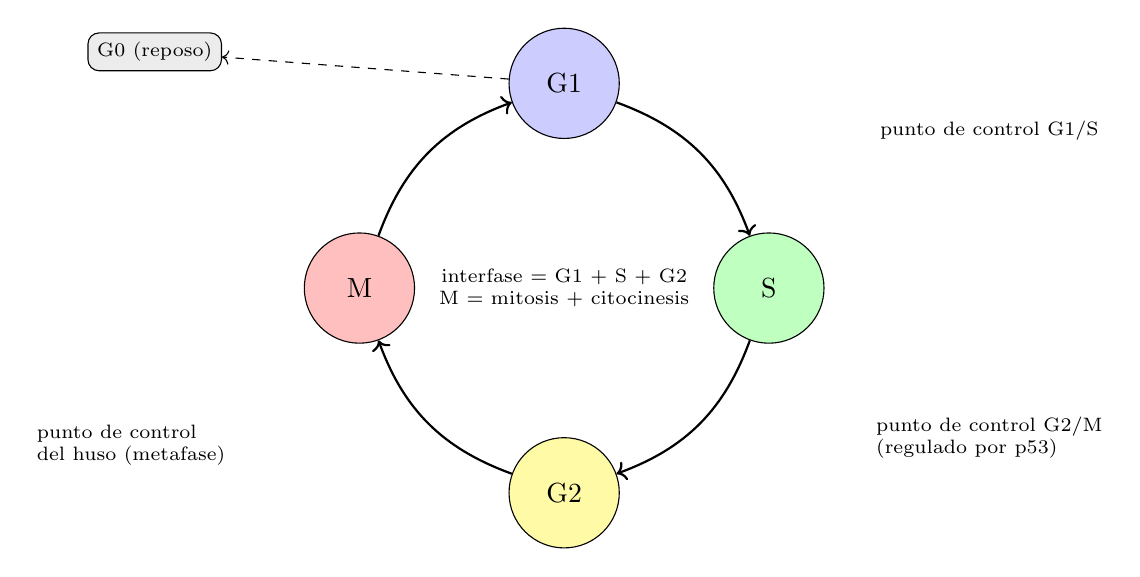
\begin{tikzpicture}
\tikzset{every node/.append style={align=center}}

\foreach \a/\t/\c in {90/G1/blue!20, 0/S/green!25, -90/G2/yellow!35, 180/M/red!25} {
  \node[draw, circle, fill=\c, minimum size=1.4cm] (n\a) at (\a:2.6) {\t};}
\draw[->, thick] (n90) to[bend left=25] (n0); \draw[->, thick] (n0) to[bend left=25] (n-90); \draw[->, thick] (n-90) to[bend left=25] (n180); \draw[->, thick] (n180) to[bend left=25] (n90);
\node[font=\scriptsize, align=center] at (0,0.0) {interfase = G1 + S + G2\\ M = mitosis + citocinesis};
\node[draw, rounded corners, fill=gray!15, font=\scriptsize] (g0) at (-5.2,3.0) {G0 (reposo)};
\draw[->, dashed] (n90) -- (g0);
\node[font=\scriptsize, align=left] at (5.4,2.0) {punto de control G1/S};
\node[font=\scriptsize, align=left] at (5.4,-1.9) {punto de control G2/M\\ (regulado por p53)};
\node[font=\scriptsize, align=left] at (-5.5,-2.0) {punto de control\\ del huso (metafase)};

\end{tikzpicture}
\end{document}
